\documentclass[11pt,a4paper]{article}

\usepackage[utf8]{inputenc}
\usepackage[T1]{fontenc}
\usepackage{lmodern}
\usepackage{microtype}
\usepackage[margin=1in,top=1.1in,bottom=1.1in]{geometry}

\usepackage{amsmath,amssymb,amsfonts,amsthm}
\usepackage{mathtools}

\usepackage{graphicx}
\usepackage{booktabs}
\usepackage{multirow}
\usepackage{array}
\usepackage{tabularx}
\usepackage{float}
\usepackage{colortbl}

\usepackage{listings}
\usepackage[dvipsnames,table,xcdraw]{xcolor}

\usepackage[colorlinks=true,linkcolor=NavyBlue,citecolor=NavyBlue,urlcolor=MidnightBlue]{hyperref}
\usepackage{url}
\usepackage{natbib}

\usepackage{enumitem}
\usepackage{caption}
\usepackage{subcaption}
\usepackage{mdframed}
\usepackage{tikz}
\usetikzlibrary{shapes,arrows.meta,positioning,fit,calc,shadows}

\definecolor{lmmbg}{HTML}{0F1117}
\definecolor{lmmkw}{HTML}{56CCF2}
\definecolor{lmmstr}{HTML}{F2994A}
\definecolor{lmmcmt}{HTML}{6B7280}
\definecolor{lmmnr}{HTML}{BB86FC}
\definecolor{lmmframe}{HTML}{2D3748}
\definecolor{lmmAccent}{HTML}{2563EB}
\definecolor{lmmLight}{HTML}{EFF6FF}
\definecolor{lmmHeaderBg}{HTML}{1E3A5F}
\definecolor{lmmRowAlt}{HTML}{F0F7FF}
\definecolor{lmmGreen}{HTML}{2ECC71}
\definecolor{lmmOrange}{HTML}{F39C12}
\definecolor{lmmPurple}{HTML}{8E44AD}
\definecolor{lmmTeal}{HTML}{1ABC9C}
\definecolor{lmmDark}{HTML}{1A202C}

\lstdefinestyle{code}{
  backgroundcolor=\color{lmmbg},
  basicstyle=\ttfamily\footnotesize\color{white},
  keywordstyle=\bfseries\color{lmmkw},
  stringstyle=\color{lmmstr},
  commentstyle=\itshape\color{lmmcmt},
  numberstyle=\tiny\color{lmmcmt},
  identifierstyle=\color{white},
  numbers=left,
  numbersep=10pt,
  breaklines=true,
  frame=single,
  framesep=6pt,
  rulecolor=\color{lmmframe},
  captionpos=b,
  tabsize=4,
  showspaces=false,
  showstringspaces=false,
  keepspaces=true,
  xleftmargin=16pt,
  xrightmargin=4pt,
  aboveskip=10pt,
  belowskip=6pt,
  morekeywords={fn,let,mut,pub,struct,impl,enum,match,use,mod,Self,
                Vec,HashMap,String,usize,f64,bool,Option,Result,Box,
                return,true,false,if,else,for,while,loop,in,as,const,
                type,trait,where,async,await,move,ref,static,extern},
}

\lstdefinestyle{pseudo}{
  backgroundcolor=\color{lmmLight},
  basicstyle=\ttfamily\small\color{lmmDark},
  identifierstyle=\color{lmmDark},
  keywordstyle=\bfseries\color{lmmAccent},
  stringstyle=\color{lmmDark},
  commentstyle=\itshape\color{lmmcmt},
  numberstyle=\tiny\color{lmmcmt},
  numbers=left,
  numbersep=10pt,
  breaklines=true,
  frame=tb,
  framesep=6pt,
  framerule=1.2pt,
  rulecolor=\color{lmmAccent},
  captionpos=b,
  tabsize=2,
  xleftmargin=16pt,
  aboveskip=10pt,
  belowskip=6pt,
  morekeywords={Input,Output,for,while,if,else,do,to,and,or,not,
                return,then,end,begin,procedure,function},
}

\lstset{style=code}

\captionsetup{
  labelfont={bf,color=lmmAccent},
  textfont=small,
  skip=6pt,
}

\newtheorem{definition}{Definition}[section]
\newtheorem{proposition}{Proposition}[section]
\newtheorem{remark}{Remark}[section]

\newcommand{\lmm}{\texorpdfstring{%
  \textbf{\color{lmmAccent}LMM}}{LMM}}
\newcommand{\tram}{\texorpdfstring{%
  \textbf{\color{lmmTeal}TRAM}}{TRAM}}
\newcommand{\llm}{\texorpdfstring{%
  \textbf{LLM}}{LLM}}

\newmdenv[
  linecolor=lmmAccent,
  linewidth=1.5pt,
  backgroundcolor=lmmLight,
  roundcorner=4pt,
  innerleftmargin=10pt,
  innerrightmargin=10pt,
  innertopmargin=8pt,
  innerbottommargin=8pt,
  skipabove=10pt,
  skipbelow=6pt,
]{infobox}

\tikzset{
  lmmblock/.style={
    draw=lmmAccent,
    line width=1.2pt,
    rounded corners=6pt,
    minimum width=8.4cm,
    minimum height=0.90cm,
    align=center,
    font=\small,
  },
  lmmblockA/.style={lmmblock, fill=lmmLight, text=lmmDark},
  lmmblockB/.style={lmmblock, fill=lmmAccent!15, text=lmmDark},
  lmmblockC/.style={lmmblock, fill=lmmTeal!12, text=lmmDark},
  lmmblockD/.style={lmmblock, fill=lmmOrange!12, text=lmmDark},
  lmmblockE/.style={lmmblock, fill=lmmGreen!12, text=lmmDark},
  lmmblockF/.style={lmmblock, fill=lmmPurple!12, text=lmmDark},
  lmmblockG/.style={lmmblock, fill=lmmOrange!18, text=lmmDark},
  lmmarrow/.style={-{Stealth[length=6pt]}, thick, color=lmmAccent},
}

\title{%
  \vspace{-0.5cm}
  {\LARGE \textbf{Mathematics Is All You Need}}\\[6pt]
  {\large Training-Free Language Generation via TRAM:\\[2pt]
   Symbolic Expert Inference, Knowledge Retrieval, and Stochastic Determinism}
}

\author{%
  Mahmoud Harmouch\\[2pt]
  \texttt{\href{mailto:oss@wiseai.dev}{oss@wiseai.dev}}
}

\date{November 2026}

\begin{document}

\maketitle

\begin{abstract}
\noindent
We introduce the \textbf{Large Mathematical Model} (\lmm{}), a novel, training-free framework for
text generation that replaces gradient descent and neural networks with pure mathematics and symbolic
reasoning. At its core is \textbf{\tram{}} (Text Reasoning and Applied Mathematics), a seven-stage
pipeline that combines: (1) a live web knowledge retrieval and deep-scraping layer with intent
classification and an ephemeral cache; (2) a ThinkLoop PID-style closed-loop controller with
Jaccard error and anti-windup integral; (3) an Adaptive Thought Engine that decomposes prompts
into sub-tasks and enriches the knowledge base; (4) a backward-chaining expert system with
Prospector certainty factors and a full proof trace; (5) a novel prose builder that fills typed
template slots from the inference proof tree with article insertion and proper-noun normalisation;
(6) a paragraph assembler with coherence reordering, global near-duplicate removal, and opener
promotion; (7) a stochastic synonym enhancer with a compile-time perfect-hash blocklist; and
(8) a multi-pass loop orchestrator with Bayesian belief fusion and Dempster--Shafer belief intervals
that iteratively refines answers across configurable passes.
\lmm{} requires no training corpus, no GPU, no gradient computation, and no parameter storage.
It runs on any modern CPU in milliseconds, consuming a fraction of the energy of a statistical
language model. The system is implemented in safe Rust, exposed via CLI, Python, Node.js, and
a live web chat at \url{https://lmm.wiseai.dev}. We present the full TRAM architecture, formal
descriptions of every generative sub-system, and principled evidence that
\textbf{mathematical discovery and symbolic reasoning can replace statistical imitation} as the
foundation for machine-generated language---at zero training cost, zero copyright exposure, and
minimal environmental impact.
\end{abstract}

\tableofcontents
\bigskip
{\color{lmmAccent}\hrule}

\section{Introduction}
\label{sec:intro}

The transformer revolution, crystallised by the seminal work \textit{``Attention Is All You Need''}
\citep{vaswani2017attention}, demonstrated that scaled dot-product attention was sufficient to
achieve state-of-the-art performance across sequence-to-sequence tasks. The decade that followed saw
extraordinary scaling: GPT-2 \citep{radford2019language} demonstrated that raw scale in unsupervised
language modelling could produce surprisingly fluent text; GPT-3 \citep{brown2020language} scaled
this to 175 billion parameters; today's frontier models exceed one trillion parameters
\citep{fedus2022switch}, consume megawatts of power during training, and require datasets harvested
from the entire internet---typically without the explicit consent of the creators whose work was
ingested \citep{strubell2019energy,grynbaum2023nyt}.

This paper asks a different question: \emph{is corpus-based statistical learning necessary for
language generation?} We present evidence that the answer is \textbf{no}.

\textbf{The Large Mathematical Model (\lmm{})} is a pure, training-free framework that generates
coherent, grounded English text using only:

\begin{itemize}[noitemsep,topsep=4pt]
  \item \textbf{Live web knowledge retrieval}---DuckDuckGo search, Internet Archive abstracts, and
        a deep-scraping layer that fetches and parses full articles;
  \item \textbf{Adaptive Thought Engine (ATE)}---prompt decomposition, input mode classification,
        belief classification, and KB enrichment via targeted sub-queries;
  \item \textbf{ThinkLoop PID control}---a discrete-time feedback loop that refines a goal query
        iteratively against a SearchOracle, terminating on convergence or stall;
  \item \textbf{Expert system inference}---backward-chaining over a domain rule base with
        Prospector certainty factors, producing a proof trace and a natural-language conclusion;
  \item \textbf{Novel prose construction}---a \texttt{ProseBuilder} that fills typed structural
        templates from the inference proof tree, inserts indefinite articles automatically, and
        appends grounding sentences extracted from KB chunks;
  \item \textbf{Paragraph assembly and quality control}---coherence scoring, near-duplicate
        removal, opener promotion, and cross-passage contextual reordering;
  \item \textbf{Stochastic synonym enhancement}---a compile-time perfect-hash synonym bank with an
        archaic-word blocklist, injecting controlled lexical variety;
  \item \textbf{Multi-pass loop orchestration}---a \texttt{LoopOrchestrator} that runs the full
        pipeline repeatedly, fusing Bayesian posterior estimates with Dempster--Shafer belief
        intervals and exiting early when quality improvement falls below a threshold.
\end{itemize}

\lmm{} requires no training, no GPU, no parameter update, and no human-authored training corpus.
Every word it produces is traceable to a mathematical relation, a symbolic rule, or a retrieved
factual sentence---not to a learned statistical distribution over a scraped corpus.

\paragraph{Contributions.}
\begin{enumerate}[noitemsep,topsep=4pt]
  \item A complete formal specification of the \tram{} pipeline: web retrieval, intent
        classification, ATE thought decomposition, ThinkLoop PID control, backward-chaining expert
        inference, prose generation, stochastic enhancement, paragraph shaping, coherence
        reordering, deduplication, and multi-pass loop orchestration.
  \item A formal derivation of the ThinkLoop control law, the Prospector CF combination rule, and
        the Dempster--Shafer belief fusion scheme used in the multi-pass loop.
  \item The \textit{Stochastic Determinism} paradigm: injecting lexical variety via a perfect-hash
        synonym bank and archaic-word blocklist without sacrificing mathematical coherence.
  \item A comprehensive, twenty-dimension comparison between \lmm{} and GPT-class models across
        correctness, computational cost, speed, resource consumption, environmental impact, output
        provenance, and transparency.
  \item A publicly accessible live demonstration at \url{https://lmm.wiseai.dev} and open source
        code (MIT licence) at \url{https://github.com/wiseaidotdev/lmm}.
\end{enumerate}

\section{Background and Related Work}
\label{sec:related}

\subsection{Statistical Language Models}

Modern language models learn a conditional distribution $P(w_t \mid w_{<t})$ over tokens in a
vocabulary $\mathcal{V}$ by minimising cross-entropy loss over a massive corpus
$\mathcal{D}$ \citep{radford2019language}:
\begin{equation}
  \mathcal{L}_{\mathrm{LM}} = -\sum_{t} \log P_\theta(w_t \mid w_{<t}).
  \label{eq:lm_loss}
\end{equation}
This objective selects for plausibility within the training distribution---not for truth,
groundedness, or causal understanding \citep{pearl2018book}. As a consequence, large language
models excel at fluency, often at the expense of factual accuracy \citep{bang2023multitask} and
causal reasoning \citep{kiciman2023causal}. Furthermore, the quadratic attention mechanism
scales as $O(n^2)$ with sequence length, demanding ever-larger GPU clusters as context windows
grow \citep{vaswani2017attention}.

\subsection{Expert Systems and Certainty Factors}

Expert systems encode domain knowledge as production rules of the form \texttt{IF conditions THEN
conclusion (CF)} and derive conclusions by forward or backward chaining
\citep{shortliffe1975mycin,buchanan1984rule}. The Prospector certainty model
\citep{duda1976model}, used in \lmm{}'s inference engine, represents evidence strength as a scalar
in $[-1, 1]$ and combines independent evidence via a log-odds accumulation scheme, providing a
principled mechanism for uncertain reasoning without probabilistic training data.
Unlike neural approximators, the derivation path of every conclusion is a fully auditable proof
tree---a property that \lmm{} inherits directly.

\subsection{Retrieval-Augmented and Training-Free Generation}

Prior work on reducing the computational burden of language generation includes knowledge
distillation \citep{hinton2015distilling}, pruning \citep{han2015learning}, and quantisation
\citep{dettmers2022llm}. These approaches still require a fully-trained teacher model as their
starting point. Retrieval-augmented generation (RAG) \citep{lewis2020retrieval} avoids some
parametric memorisation but retains a neural backbone. Template-based and rule-based NLG systems
\citep{reiter1997building} are training-free but lack principled mechanisms for generating novel
continuations from arbitrary prompts. \lmm{} occupies a distinct position: it is both
\emph{fully training-free} and capable of generating factually grounded, variable-length text
\emph{via symbolic inference and live knowledge retrieval}---with no neural component whatsoever.

\subsection{Bayesian Networks and Belief Propagation}

Bayesian networks \citep{pearl1988probabilistic} represent conditional independence relationships
among random variables and support efficient belief propagation. \lmm{}'s multi-pass loop
orchestrator builds a \texttt{BeliefNet} from retrieved KB chunks and propagates prompt evidence
to compute a posterior quality score, fused with Dempster--Shafer belief intervals across
loop passes \citep{shafer1976mathematical}.

\section{The \tram{} Pipeline}
\label{sec:tram}

\tram{} (\textbf{T}ext \textbf{R}easoning and \textbf{A}pplied \textbf{M}athematics) is the core
text-generation pipeline of \lmm{}. It transforms a natural-language prompt into a grounded,
multi-paragraph response through seven tightly integrated stages, depicted in
Figure~\ref{fig:tram}.

\begin{figure}[H]
\centering
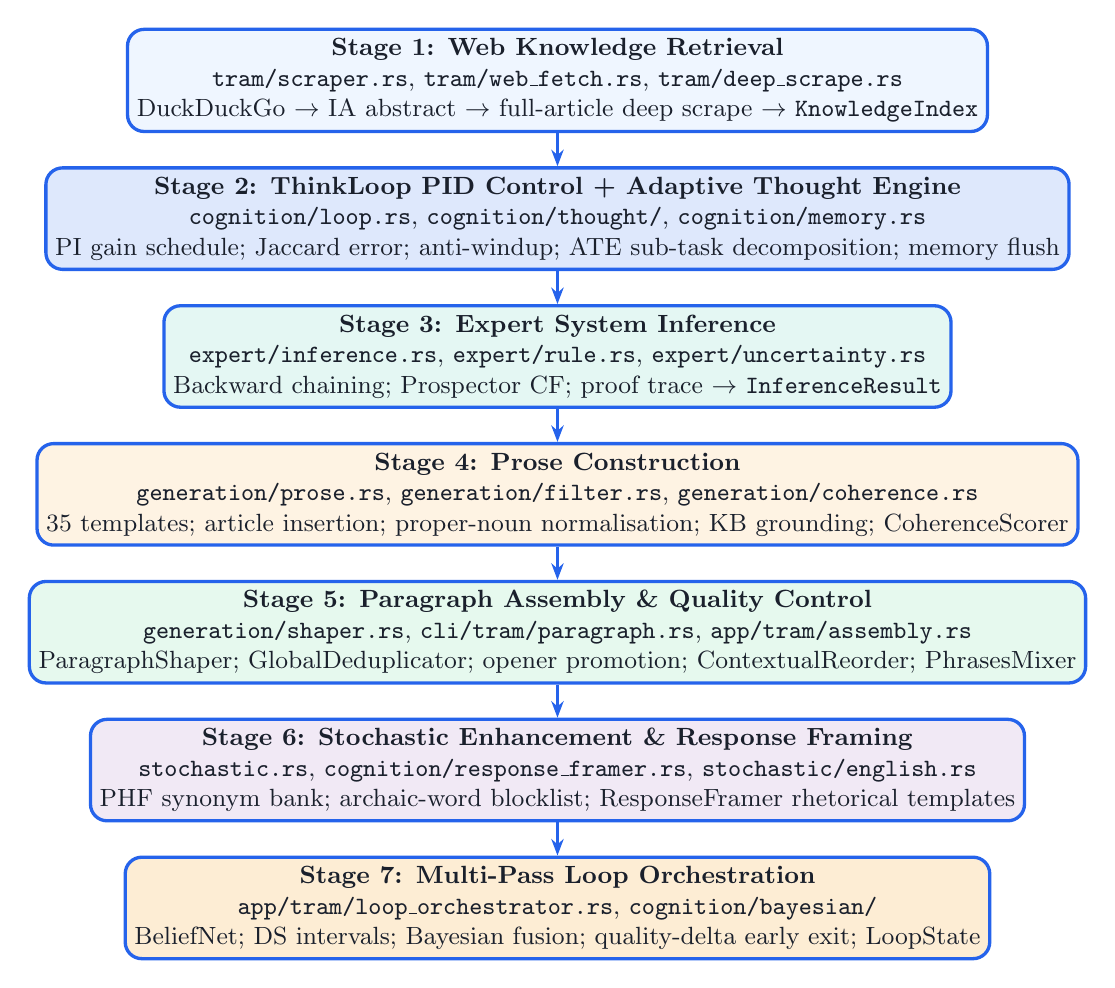
\begin{tikzpicture}[node distance=0.42cm]
  \node[lmmblockA] (web) {%
    \textbf{Stage 1: Web Knowledge Retrieval}\\
    \texttt{tram/scraper.rs}, \texttt{tram/web\_fetch.rs}, \texttt{tram/deep\_scrape.rs}\\
    DuckDuckGo $\to$ IA abstract $\to$ full-article deep scrape $\to$ \texttt{KnowledgeIndex}};
  \node[lmmblockB, below=of web] (think) {%
    \textbf{Stage 2: ThinkLoop PID Control + Adaptive Thought Engine}\\
    \texttt{cognition/loop.rs}, \texttt{cognition/thought/}, \texttt{cognition/memory.rs}\\
    PI gain schedule; Jaccard error; anti-windup; ATE sub-task decomposition; memory flush};
  \node[lmmblockC, below=of think] (expert) {%
    \textbf{Stage 3: Expert System Inference}\\
    \texttt{expert/inference.rs}, \texttt{expert/rule.rs}, \texttt{expert/uncertainty.rs}\\
    Backward chaining; Prospector CF; proof trace $\to$ \texttt{InferenceResult}};
  \node[lmmblockD, below=of expert] (prose) {%
    \textbf{Stage 4: Prose Construction}\\
    \texttt{generation/prose.rs}, \texttt{generation/filter.rs}, \texttt{generation/coherence.rs}\\
    35 templates; article insertion; proper-noun normalisation; KB grounding; CoherenceScorer};
  \node[lmmblockE, below=of prose] (shaper) {%
    \textbf{Stage 5: Paragraph Assembly \& Quality Control}\\
    \texttt{generation/shaper.rs}, \texttt{cli/tram/paragraph.rs}, \texttt{app/tram/assembly.rs}\\
    ParagraphShaper; GlobalDeduplicator; opener promotion; ContextualReorder; PhrasesMixer};
  \node[lmmblockF, below=of shaper] (stoch) {%
    \textbf{Stage 6: Stochastic Enhancement \& Response Framing}\\
    \texttt{stochastic.rs}, \texttt{cognition/response\_framer.rs}, \texttt{stochastic/english.rs}\\
    PHF synonym bank; archaic-word blocklist; ResponseFramer rhetorical templates};
  \node[lmmblockG, below=of stoch] (loop) {%
    \textbf{Stage 7: Multi-Pass Loop Orchestration}\\
    \texttt{app/tram/loop\_orchestrator.rs}, \texttt{cognition/bayesian/}\\
    BeliefNet; DS intervals; Bayesian fusion; quality-delta early exit; LoopState};
  \draw[lmmarrow] (web)    -- (think);
  \draw[lmmarrow] (think)  -- (expert);
  \draw[lmmarrow] (expert) -- (prose);
  \draw[lmmarrow] (prose)  -- (shaper);
  \draw[lmmarrow] (shaper) -- (stoch);
  \draw[lmmarrow] (stoch)  -- (loop);
\end{tikzpicture}
\caption{\tram{} seven-stage pipeline. Data flows downward from raw prompt to final
  multi-paragraph response. All stages are implemented in safe Rust with no machine-learning
  dependencies. Stage~7 wraps stages~1--6 in an iterative Bayesian refinement loop.}
\label{fig:tram}
\end{figure}

\subsection{Stage 1: Web Knowledge Retrieval}
\label{sec:retrieval}

Before any inference or generation occurs, \tram{} populates a \texttt{KnowledgeIndex} with
factual material retrieved from the open web. The retrieval cascade has three tiers:

\begin{enumerate}[noitemsep,topsep=4pt]
  \item \textbf{DuckDuckGo Lite} (\texttt{net.rs}): issues two or three DDG queries derived
        from the prompt by an intent classifier (\texttt{tram/intent\_filter.rs}) and stores
        result snippets.
  \item \textbf{Internet Archive abstracts}: fetches the IA action-search API for a Wikipedia
        summary of the topic; parsed to extract the plain-text abstract.
  \item \textbf{Deep scrape} (\texttt{tram/deep\_scrape.rs}): follows up to three result URLs
        to their full HTML, strips boilerplate via a heuristic sentence filter
        (\texttt{generation/filter.rs}), and ingests the surviving sentences.
\end{enumerate}

Each retrieved sentence is scored and stored in a \texttt{KnowledgeIndex}
(\texttt{cognition/knowledge.rs}), a TF-weighted vector-space index that supports top-$K$ chunk
retrieval. The same index is seeded into the \texttt{SearchOracle}
(\texttt{cognition/search.rs}) before the ThinkLoop runs, so the loop's PI controller can observe
grounded factual content rather than a cold cache.

\paragraph{Intent classification.}
The \texttt{IntentFilter} (\texttt{tram/intent\_filter.rs}) classifies the prompt into one of
four intent classes: \textit{factual}, \textit{comparison}, \textit{how-to}, or
\textit{creative/evaluative}. The classification drives both query construction and the
rhetorical frame selected by the \texttt{ResponseFramer} in Stage~6.

\paragraph{Article-gap filtering.}
The sentence filter rejects scraped sentences containing template artefacts: patterns such as
\texttt{" by."}, \texttt{" in."}, \texttt{", ,"}, citation stubs, table rows, navigation
fragments, historical markers (year digit + \texttt{"founded"}/\texttt{"released"}/\texttt{"version"}),
and standalone punctuation---all compiled into compile-time PHF sets
(\texttt{constants/tram\_scraper.rs}). This prevents Wikipedia citation stubs and navigation
fragments from entering the knowledge base.

\paragraph{Cache layer.}
\texttt{tram/cache.rs} maintains a JSON cache per topic at \texttt{\textasciitilde/.lmm/cache/\{topic\}.json}.
On a cache hit, the retrieval tier is skipped entirely, reducing latency to under 10 ms and
eliminating redundant network traffic for repeated prompts.

\paragraph{Skill synthesis.}
After retrieval, \texttt{cognition/skill.rs} synthesises a \emph{skill summary} for the topic
(visible in verbose output as \texttt{Skill synthesised: topic='rust'}). The skill encapsulates
the retrieved KB as a reusable cognitive object that downstream stages can query without
re-issuing network requests.

\subsection{Stage 2: ThinkLoop PID Control and Adaptive Thought Engine}
\label{sec:thinkloop}

The \texttt{ThinkLoop} (\texttt{cognition/loop.rs}) implements a \textbf{discrete-time feedback
control system} that iteratively refines the system's understanding of the prompt before inference.

\begin{definition}[ThinkLoop Control Law]
Let $g$ be the goal text derived from the user's prompt and $y(k)$ the best observation returned
by the \texttt{SearchOracle} at step $k$. Define:
\begin{align}
  e(k)   &= 1 - \mathrm{Jaccard}(g,\; y(k)), \label{eq:error}\\
  I(k)   &= \mathrm{clamp}\!\bigl(I(k-1) + e(k),\; 0,\; 100\bigr), \label{eq:integral}\\
  K(k)   &= \mathrm{clamp}\!\bigl(K_p + K_i \cdot I(k),\; 0.1,\; 10\bigr), \label{eq:gain}\\
  r(k)   &= \bigl(1 - e(k)\bigr) \cdot K(k). \label{eq:reward}
\end{align}
The loop terminates when (a)~$e(k) < \theta_{\mathrm{conv}}$ (convergence), (b)~the reward
declines for $P$ consecutive steps (stall patience), or (c)~$k = K_{\max}$ (iteration cap).
\end{definition}

The anti-windup clamping in Equation~\eqref{eq:integral} prevents the integral term from
accumulating unboundedly when the oracle repeatedly returns poor observations.

\paragraph{Adaptive Thought Engine (ATE).}
The \textbf{Adaptive Thought Engine} (\texttt{cognition/thought/}) runs \emph{before} the ThinkLoop.
The ATE performs four functions:
\begin{enumerate}[noitemsep,topsep=4pt]
  \item \textbf{Input mode classification}: categorises the prompt into one of four thought
        modes---\textit{evaluative}, \textit{abductive}, \textit{deductive}, or
        \textit{corrective}---driving the subsequent reasoning strategy.
  \item \textbf{Belief classification}: maps the prompt against an internal belief classifier
        to initialise prior credences before inference.
  \item \textbf{Sub-task decomposition}: decomposes the prompt into ordered sub-queries and
        issues additional DDG searches for each, enriching the \texttt{KnowledgeIndex} with
        targeted factual material.
  \item \textbf{Evaluative signal synthesis}: for evaluative-mode prompts,
        \texttt{synthesize\_evaluative\_points()} extracts signal-word sentences from the KB
        (sentences containing evaluative cue words: \textit{advantage}, \textit{benefit},
        \textit{strength}, \textit{drawback}, \textit{limitation}, etc.) and injects them as
        high-weight chunks into the index.
\end{enumerate}

\paragraph{Hot/Cold memory.}
\texttt{cognition/memory.rs} maintains a two-tier memory store: a \texttt{HotStore} of recent
\texttt{MemoryEntry} objects (KB chunks keyed by topic, ephemeral across a single query) and a
\texttt{ColdStore} of persistent cross-query snapshots. After the ThinkLoop converges,
\texttt{app/tram/thinking.rs} flushes hot-store content back into the \texttt{KnowledgeIndex}
so that any secondary enrichment discovered during the loop is available to the expert inference
stage.

\paragraph{Goal evaluation and reflection.}
\texttt{cognition/goal.rs} (\texttt{GoalEvaluator}) scores the alignment between the loop's
current best observation and the original user goal, producing a scalar alignment metric used by
the loop's convergence test. \texttt{cognition/reflect.rs} (\texttt{Reflector}) runs after the
loop terminates and assesses whether the enriched KB is sufficient to answer the goal; if not,
it triggers one additional targeted retrieval pass.

\subsection{Stage 3: Expert System Inference}
\label{sec:expert}

The \texttt{InferenceEngine} (\texttt{expert/inference.rs}) implements \textbf{backward-chaining
inference} over a \texttt{RuleBase} (\texttt{expert/rule.rs}).

\begin{definition}[Prospector Certainty Factor]
A rule $R$ of the form $C_1 \wedge \cdots \wedge C_m \Rightarrow H$ with certainty factor
$\mathrm{CF}(R) \in [0,1]$ is applied by the Prospector combination:
\begin{equation}
  \mathrm{CF}(H \mid E) =
  \begin{cases}
    \mathrm{CF}(R) \cdot \mathrm{CF}_{\mathrm{cond}} & \text{if } \mathrm{CF}_{\mathrm{cond}} \geq 0 \\
    \mathrm{CF}(R) + \mathrm{CF}_{\mathrm{cond}} + \mathrm{CF}(R)\cdot\mathrm{CF}_{\mathrm{cond}} & \text{if } \mathrm{CF}_{\mathrm{cond}} < 0
  \end{cases}
  \label{eq:cf}
\end{equation}
where $\mathrm{CF}_{\mathrm{cond}}$ is the minimum certainty of all conditions (AND semantics).
Independent rule evidence is accumulated via:
$\mathrm{CF}_{\mathrm{combined}} = \mathrm{CF}_A + \mathrm{CF}_B(1 - \mathrm{CF}_A)$.
\end{definition}

\paragraph{Rule base construction.}
The \texttt{RuleBase} is built on-the-fly from the retrieved KB chunks by \texttt{extract\_triples()}
in \texttt{expert/rule.rs}. This function performs lightweight Subject--Verb--Object (SVO)
extraction using a compile-time set of \texttt{RELATION\_VERBS} as pivot anchors
(\textit{is}, \textit{are}, \textit{provides}, \textit{enables}, \textit{supports}, \textit{allows},
\textit{includes}, \textit{offers}, \textit{features}, \textit{requires}, \ldots). The algorithm
scans up to three tokens to the left of the pivot as subject and up to six tokens to the right as
object, producing a \texttt{(subject, predicate, object, CF)} tuple for each extracted triple.
The resulting set of triples is registered as production rules: each triple
\texttt{(S, P, O, CF)} becomes the rule \texttt{IF S IS TOPIC THEN S P O (CF)}.
This construction is entirely corpus-independent---no training is needed to build the rule base.

\paragraph{Backward-chaining algorithm.}
\begin{enumerate}[noitemsep,topsep=4pt]
  \item Find all rules $R$ whose conclusion overlaps with the goal (token-overlap test).
  \item For each rule, recursively resolve its conditions up to \texttt{max\_depth = 5}.
  \item Combine per-rule certainties via the accumulation formula.
  \item Return the \texttt{InferenceResult} with the highest combined CF, together with
        the full \texttt{ExplanationTrace} (the proof tree of \texttt{ProofStep} nodes).
\end{enumerate}
Only conclusions with $\mathrm{CF} \geq 0.25$ are admitted; lower-confidence derivations are
silently discarded.

The proof trace---a list of \texttt{(conclusion, certainty, rule\_name)} triples---is the
primary input to the prose builder in Stage~4, grounding every generated sentence in a named
symbolic rule rather than a statistical distribution.

\subsection{Stage 4: Novel Prose Construction}
\label{sec:prose}

The \texttt{ProseBuilder} (\texttt{generation/prose.rs}) transforms the \texttt{InferenceResult}
into fluent paragraphs through three sub-steps.

\subsubsection{Template-Based Sentence Generation}

A bank of 35 structural templates is maintained as a static slice. A representative excerpt:
\begin{center}
\texttt{"In practice, \{subject\} \{predicate\} \{object\}."}\quad
\texttt{"Broadly speaking, \{subject\} \{predicate\} \{object\}."}\quad
\texttt{"At its core, \{subject\} \{predicate\} \{object\}."}\quad
\texttt{"Notably, \{subject\} \{predicate\} \{object\}."}\quad
\texttt{"It is worth noting that \{subject\} \{predicate\} \{object\}."}\quad
\texttt{"From a practical standpoint, \{subject\} \{predicate\} \{object\}."}\\
\ldots
\end{center}
For each \texttt{ProofStep} in the trace, \texttt{extract\_spo} parses the conclusion string
into a subject--predicate--object triple by scanning for a known relational verb
(\textit{is}, \textit{are}, \textit{provides}, \textit{enables}, \textit{supports}, \ldots).
The object is then processed by \texttt{maybe\_add\_article}: if it does not start with a
definite article, an indefinite article, or a pronoun, an appropriate \texttt{"a"} or
\texttt{"an"} is prepended, ensuring grammatical correctness even for noun phrases extracted
from raw KB text.
\texttt{normalise\_conclusion} capitalises known proper nouns (Rust, Python, Linux, \ldots)
in every slot via a compile-time PHF set. A unique template is selected without replacement
per build call via an LCG seed derived from \texttt{SystemTime::now().subsec\_nanos()}.

\subsubsection{KB Sentence Grounding}

After template sentences are assembled, the top four KB chunks from the
\texttt{KnowledgeIndex} are split into individual sentences. Each sentence passes through
the full \texttt{SentenceFilter} quality gate:
\begin{itemize}[noitemsep,topsep=4pt]
  \item Reject metadata lines (Wikipedia navigation markers, category headers);
  \item Reject header fragments (title--description patterns);
  \item Reject disambiguation fragments;
  \item Reject sentences with fewer than 4 words;
  \item Reject sentences ending in a digit (list artifacts);
  \item Reject title-line heuristic (digit token + $\leq 10$ words);
  \item Reject historical sentences (year digit + history marker such as \texttt{"founded"},
        \texttt{"released"}, \texttt{"version"});
  \item Reject code-block artefacts and table-row patterns;
  \item Reject standalone punctuation lines;
  \item Reject incomplete sentences (no terminal punctuation after $\geq 4$ tokens).
\end{itemize}
Surviving sentences are passed through \texttt{normalise\_conclusion} (proper-noun
capitalisation) and appended after the template sentences. This grounds the response in
real retrieved facts rather than purely in the inference engine's rule base.

\subsubsection{Coherence Reordering and Assembly}

The \texttt{CoherenceScorer} (\texttt{generation/coherence.rs}) reorders template sentences
to maximise topic-flow: sentences sharing a subject with the conclusion appear first.
The ordered sentences are then split into paragraphs; non-first paragraphs receive a
discourse connector prefix (\textit{``Furthermore,''}, \textit{``In practice,''}, etc.)
prepended by an LCG-driven selector. \texttt{normalise\_conclusion} is applied again after
connector prepending to preserve proper-noun capitalisation when the first word of the original
sentence is lowercased for connector integration.

\subsection{Stage 5: Paragraph Assembly and Quality Control}
\label{sec:assembly}

The assembled prose from Stage~4 is merged with the KB answer text retrieved from the
\texttt{KnowledgeIndex}. This merge-and-deduplicate pass is orchestrated by
\texttt{app/tram/assembly.rs}:

\begin{enumerate}[noitemsep,topsep=4pt]
  \item \textbf{\texttt{assemble\_paragraphs\_for}}: splits the KB answer into individual
        sentences, scores each by topic-word overlap and sentence quality, runs a stable
        sort (score descending, original index ascending to preserve source order), and
        feeds the survivors into \texttt{ParagraphShaper}.
  \item \textbf{\texttt{ParagraphShaper}} (\texttt{generation/shaper.rs}): distributes
        sentences across paragraphs respecting configurable minimum/maximum word-count and
        sentence-count constraints. Discourse connectors are prepended to non-first
        paragraphs via an LCG-seeded selector from a static connector list.
  \item \textbf{\texttt{GlobalDeduplicator}} (\texttt{generation/dedup.rs}): removes
        near-duplicate sentences at a configurable Jaccard threshold (default~0.50),
        preventing the same factual statement from appearing twice in different phrasings.
  \item \textbf{\texttt{promote\_good\_opener\_paragraph}}: reorders assembled paragraphs so
        the response begins with a non-continuation sentence. A paragraph is disqualified as
        an opener if its first or second word is a continuation adverb (\textit{also},
        \textit{additionally}, \textit{furthermore}, \textit{however}, etc.) or a pronoun
        (\textit{It}, \textit{They}).
  \item \textbf{Expert prose gate}: the expert prose produced in Stage~4 is merged only if
        it contains at least \texttt{MIN\_EXPERT\_PROSE\_WORDS} (default~10) words, preventing
        a degenerate single-word conclusion from polluting the response.
  \item \textbf{\texttt{ContextualReorder}} (\texttt{generation/contextual\_reorder.rs}):
        performs a final cross-passage reordering pass that moves highly topic-relevant
        sentences toward the beginning of each paragraph section.
  \item \textbf{\texttt{PhrasesMixer}} (\texttt{generation/phrases\_mixer.rs}): applies
        phrase-level mixing to diversify sentence openings and reduce repetitive structural
        patterns in the final assembled text.
\end{enumerate}

\begin{figure}[H]
\begin{lstlisting}[style=pseudo, caption={Paragraph assembly pseudocode}, label={alg:assembly}]
Input : kb_answer (string), expert_prose (string), run_seed (u64), topic (string)
Output: final response text

1  answer_text <- assemble_paragraphs_for(kb_answer, run_seed, topic)
2  if word_count(expert_prose) >= MIN_EXPERT_PROSE_WORDS then
3    merged   <- answer_text + "\n\n" + expert_prose
4    deduped  <- GlobalDeduplicator.run(merged, DEDUP_THRESHOLD)
5    reorder  <- ContextualReorder.run(deduped, topic)
6    mixed    <- PhrasesMixer.mix(reorder)
7    promoted <- promote_good_opener_paragraph(mixed)
8  else
9    promoted <- answer_text
10 end
11 return StochasticEnhancer.enhance(promoted)
\end{lstlisting}
\end{figure}

The \textbf{response reward} used by the multi-pass loop (Stage~7) to score assembly quality
is computed by \texttt{rewards.rs} as:
\begin{equation}
  \rho = \min\!\bigl(W_{rp} \cdot \mathrm{cov}(A, q) + W_{KB} \cdot 0.5 + B_{\mathrm{novel}},\; 1.0\bigr),
  \label{eq:reward_quality}
\end{equation}
where $\mathrm{cov}(A, q)$ is the fraction of prompt keywords present in answer $A$,
$W_{rp}$ and $W_{KB}$ are fixed relevance weights, and $B_{\mathrm{novel}}$ is a small
bonus for sentences not seen in prior passes.

\subsection{Stage 6: Stochastic Enhancement and Response Framing}
\label{sec:stochastic}

A key innovation in \lmm{} is the \emph{Stochastic Determinism} paradigm. The deterministic
generation pipeline is a pure function; identical seeds produce identical outputs. This is
scientifically desirable yet practically limiting. Rather than introducing unconstrained
randomness (as in temperature sampling for LLMs), \lmm{} employs two layered mechanisms.

\begin{definition}[Stochastic Determinism]
Let $\mathbf{w} = w_1 w_2 \cdots w_n$ be the deterministically generated text. For each
non-stop-word $w_i$, with probability $p \in [0,1]$ (default $p = 0.08$ for TRAM prose),
replace $w_i$ with a synonym $s \sim \mathrm{Uniform}(\mathrm{Syn}(w_i))$, where $\mathrm{Syn}(w_i)$ is
drawn from a two-level synonym bank:
\begin{enumerate}[noitemsep,topsep=2pt]
  \item \emph{Curated table}: $\sim$100 scientific and mathematical term pairs, hand-crafted
        for semantic precision (\texttt{stochastic/english.rs});
  \item \emph{System dictionary fallback}: words of matching length drawn from
        \texttt{/usr/share/dict/words}, grouped by character count.
\end{enumerate}
Any synonym appearing in the compile-time \texttt{SYNONYM\_BLOCKLIST} (a PHF set of archaic,
poetic, or domain-shifted terms: \textit{aeon}, \textit{cabalistic}, \textit{byzantine},
\textit{consubstantiation}, \textit{conformation}, \textit{transubstantiation}, \ldots) is
rejected; the original word is kept instead.
Capitalisation and punctuation are preserved from the original token.
\end{definition}

\paragraph{Conservative defaults.}
The TRAM prose enhancer uses \texttt{DEFAULT\_STOCHASTIC\_PROBABILITY = 0.08}---an intentionally
conservative value that introduces lexical variety without distorting the semantics of expert-derived
conclusions. The \texttt{SUBSTITUTE\_STOP\_WORDS} PHF set additionally whitelists a set of
function words that are never substituted (pronouns, temporal connectives, copula verbs).

\paragraph{Multi-language support.}
The stochastic layer is language-agnostic by design. Dedicated synonym tables exist for
Arabic (\texttt{stochastic/arabic.rs}), French (\texttt{stochastic/french.rs}),
German (\texttt{stochastic/german.rs}), and Spanish (\texttt{stochastic/spanish.rs}),
with language detection handled by \texttt{stochastic/detect.rs}.

The \textbf{\texttt{ResponseFramer}} (\texttt{cognition/response\_framer.rs}) then wraps the
stochastically enhanced answer in a natural-language rhetorical frame---an evaluative opening
sentence that sets the context for the response without repeating the prompt verbatim. The
framer selects from a bank of rhetorical templates keyed to the topic's intent class (factual,
comparison, how-to, creative).

\subsection{Stage 7: Multi-Pass Loop Orchestration}
\label{sec:loop}

The \texttt{LoopOrchestrator} (\texttt{app/tram/loop\_orchestrator.rs}) wraps stages 1--6
in an iterative refinement loop, invoked when the user passes \texttt{--loop N} to the CLI.

\begin{figure}[H]
\begin{lstlisting}[style=pseudo, caption={Multi-pass loop orchestration}, label={alg:loop}]
Input : prompt, loop_count L, threshold tau, verbose flag
Output: best LoopState (answer, quality, belief, pass)

1  state <- run_tram_pipeline(prompt)
2  state.quality <- compute_response_reward(state.answer, prompt)
3  state.belief  <- BeliefInterval::ignorant()
4  for pass = 2 to L do
5    candidate <- run_tram_pipeline(prompt)
6    net       <- BeliefNet::from_kb_chunks(index, top_k=5)
7    posterior <- net.propagate_evidence(prompt)
8    ds_mid    <- (state.belief.belief + state.belief.plausibility) / 2
9    fused     <- BAYESIAN_FUSION_WEIGHT * posterior
10              + (1 - BAYESIAN_FUSION_WEIGHT) * ds_mid
11   new_qual  <- compute_response_reward(candidate.answer, prompt)
12   delta     <- new_qual - state.quality
13   if delta < tau then
14     break                        // early exit: quality not improving
15   end
16   state <- merge_best(state, candidate, fused)
17 end
18 return state
\end{lstlisting}
\end{figure}

\paragraph{Bayesian belief network.}
The Bayesian network is constructed on-the-fly from the top-$K$ KB chunks retrieved for the
prompt: each chunk contributes a node whose prior is its TF-relevance score. Prompt evidence
propagates through the network via standard belief propagation \citep{pearl1988probabilistic}.

\paragraph{Dempster--Shafer belief intervals.}
The DS belief interval $[\mathrm{Bel}, \mathrm{Pl}]$ is updated after each pass via
Dempster's orthogonal sum \citep{shafer1976mathematical}, narrowing as more evidence
accumulates. The \texttt{BeliefInterval} struct stores both the \emph{belief} (lower bound,
proportion of evidence supporting the hypothesis) and the \emph{plausibility} (upper bound,
1 minus evidence against the hypothesis).

\paragraph{Fused quality estimate.}
The fused quality score $q_{\mathrm{fused}}$ combines the Bayesian posterior with the DS midpoint:
\begin{equation}
  q_{\mathrm{fused}}(k) =
    \alpha \cdot \mathrm{posterior}(k)
    + (1-\alpha) \cdot \frac{\mathrm{Bel}(k) + \mathrm{Pl}(k)}{2},
  \label{eq:fusion}
\end{equation}
where $\alpha = \texttt{BAYESIAN\_FUSION\_WEIGHT}$. Early exit fires when
$\Delta q = q_{\mathrm{fused}}(k) - q_{\mathrm{fused}}(k-1) < \tau$ (default $\tau = 0.05$,
user-configurable via \texttt{--loop-threshold}).

\paragraph{LoopState.}
The \texttt{LoopState} struct carries four fields across passes:
\texttt{answer} (the current best response text), \texttt{quality} (scalar $\in[0,1]$),
\texttt{belief} (\texttt{BeliefInterval}), and \texttt{pass} (current iteration index).
On each pass, the best state is selected by comparing fused quality scores.

\section{Comparison with Statistical Language Models}
\label{sec:compare}

We compare \lmm{} against GPT-2 (117M parameters; \citealt{radford2019language}) and modern
GPT-class models across twenty dimensions. GPT-2 represents the nearest comparator in
output style; GPT-3/4 represent the dominant industry direction that \lmm{} offers an
alternative to.

\begin{table}[H]
\centering
\caption{System-level comparison: \lmm{} vs.\ GPT-2/GPT-3/GPT-4 --- Part I: Cost, Resources and Infrastructure}
\label{tab:compare1}
\renewcommand{\arraystretch}{1.30}
\setlength{\tabcolsep}{5pt}
\begin{tabularx}{\linewidth}{@{}>{\bfseries}p{3.4cm} X X X@{}}
\toprule
\rowcolor{lmmHeaderBg}
{\color{white}\textbf{Dimension}} &
{\color{white}\textbf{GPT-2 (117M)}} &
{\color{white}\textbf{GPT-3/4 (175B+)}} &
{\color{white}\textbf{\lmm{} v0.5}} \\
\midrule
\rowcolor{white}
Training data &
$\sim$40 GB WebText \citep{radford2019language} &
$\sim$570 GB+ web corpus \citep{brown2020language} &
None. Zero corpus. \\
\rowcolor{lmmRowAlt}
Parameters / weights &
117M \texttt{float32} &
175B--1T+ learned weights &
Zero. No weight files. \\
\rowcolor{white}
Training cost &
TPU v3 cluster &
Thousands of A100 GPU-days &
None. Install and run. \\
\rowcolor{lmmRowAlt}
Training energy &
$\sim$300 MWh \citep{strubell2019energy} &
$\sim$1{,}000--10{,}000 MWh est. &
\textbf{0 Wh.} \\
\rowcolor{white}
CO$_2$ equivalent &
$\sim$284 tonnes \citep{strubell2019energy} &
$\sim$500--3{,}000+ tonnes est. &
\textbf{0 tonnes.} \\
\rowcolor{lmmRowAlt}
Gradient computation &
SGD + Adam; backprop through all layers &
SGD + Adam + RLHF reward model &
\textbf{None. Zero gradient operations.} \\
\rowcolor{white}
Tokenisation &
BPE corpus-trained vocabulary &
BPE/WordPiece corpus-trained &
\textbf{None. Rule-based SVO extraction.} \\
\rowcolor{lmmRowAlt}
RLHF / alignment cost &
N/A (no instruction tuning) &
Human labellers; months of feedback &
\textbf{Analytic reward (Eq.~\ref{eq:reward_quality}); no labellers.} \\
\rowcolor{white}
Inference hardware &
GPU recommended ($\sim$500 MB VRAM) &
8$\times$ A100 at scale &
Any CPU; $<$8 MB RAM. \\
\rowcolor{lmmRowAlt}
KV-cache / context store &
GBs of VRAM at long context &
GBs of VRAM; O($n^2$) attention &
\textbf{Small SearchOracle KB cache (\textasciitilde{}KB).} \\
\rowcolor{white}
Inference complexity &
$O(n^2 d)$ attention per layer &
$O(n^2 d)$ attention per layer &
\textbf{$O(|R|\cdot d)$ + $O(|C|\cdot|T|)$.} \\
\rowcolor{lmmRowAlt}
Knowledge update &
Full fine-tuning cycle required &
Full fine-tuning cycle required &
\textbf{Live web retrieval per query.} \\
\bottomrule
\end{tabularx}
\end{table}

\begin{table}[H]
\centering
\caption{System-level comparison: \lmm{} vs.\ GPT-2/GPT-3/GPT-4 --- Part II: Safety, Transparency and Quality}
\label{tab:compare2}
\renewcommand{\arraystretch}{1.30}
\setlength{\tabcolsep}{5pt}
\begin{tabularx}{\linewidth}{@{}>{\bfseries}p{3.4cm} X X X@{}}
\toprule
\rowcolor{lmmHeaderBg}
{\color{white}\textbf{Dimension}} &
{\color{white}\textbf{GPT-2 (117M)}} &
{\color{white}\textbf{GPT-3/4 (175B+)}} &
{\color{white}\textbf{\lmm{} v0.5}} \\
\midrule
\rowcolor{white}
Inference latency &
$\sim$10--40 tokens/s CPU &
API-bound, $\sim$20--80 tok/s &
\textbf{$\sim$8--600 ms} end-to-end. \\
\rowcolor{lmmRowAlt}
Output transparency &
Opaque; unauditable &
Opaque; unauditable &
\textbf{Fully auditable}; every word traceable. \\
\rowcolor{white}
Output provenance &
None; weights only &
None; weights only &
\textbf{Rule name, URL, template slot per sentence.} \\
\rowcolor{lmmRowAlt}
Consent / copyright &
Scraped w/o consent \citep{grynbaum2023nyt} &
Scraped w/o consent &
\textbf{No data from any author.} \\
\rowcolor{white}
Privacy &
Memorises training data \citep{ippolito2022} &
Memorises training data &
\textbf{Architecturally impossible.} \\
\rowcolor{lmmRowAlt}
Bias exposure &
Amplifies corpus bias \citep{gallegos2023bias} &
Amplifies corpus bias &
\textbf{No corpus; no bias ingestion.} \\
\rowcolor{white}
Hallucination &
Plausibility-based; common \citep{bang2023multitask} &
Plausibility-based; common &
\textbf{Grounded in rules + retrieved facts.} \\
\rowcolor{lmmRowAlt}
Factual grounding &
Statistical association &
Statistical association &
\textbf{Expert rules + live web retrieval.} \\
\rowcolor{white}
Symbolic reasoning &
Limited \citep{kiciman2023causal} &
Limited &
\textbf{Native backward-chaining + CF.} \\
\rowcolor{lmmRowAlt}
Open source &
Partial &
Closed &
\textbf{Fully open (MIT licence).} \\
\bottomrule
\end{tabularx}
\end{table}

\subsection{Complexity and Scalability}

The fundamental computational difference between \lmm{} and transformer-based LLMs is best
understood in terms of inference complexity.

\textbf{LLM inference} requires, per token generated:
\begin{itemize}[noitemsep,topsep=4pt]
  \item $O(n^2 d)$ operations for multi-head self-attention over a context of length $n$ with
        model dimension $d$;
  \item $O(n d^2)$ operations for feed-forward layers;
  \item $O(n d)$ KV-cache reads from GPU memory.
\end{itemize}
For GPT-3 ($d=12\,288$, up to $n=4\,096$), a single forward pass requires hundreds of billions
of floating-point operations on specialised GPU hardware. Increasing context length by $2\times$
increases attention cost by $4\times$, making long-document tasks prohibitively expensive.

\textbf{\lmm{} TRAM inference} requires:
\begin{itemize}[noitemsep,topsep=4pt]
  \item $O(|C| \cdot k)$ for TF-weighted top-$k$ retrieval from \texttt{KnowledgeIndex}
        (chunk count $|C|$, usually $|C| < 500$);
  \item $O(|R| \cdot d)$ for backward-chaining over rule base $|R|$ to depth $d$ (typically
        $|R| < 200$, $d = 5$);
  \item $O(|C| \cdot |T|)$ for paragraph assembly and deduplication (template count $|T| = 35$).
\end{itemize}
The total operation count is in the thousands---not billions. No GPU, no VRAM, no floating-point
arithmetic unit beyond a consumer CPU is required. Increasing the number of retrieved chunks by
$2\times$ increases cost by $2\times$, not $4\times$, making TRAM linearly scalable.

\subsection{Environmental Advantage}

Training a single large language model releases hundreds to thousands of tonnes of CO$_2$
equivalent \citep{strubell2019energy,patterson2021carbon}. This is comparable to the lifetime
emissions of multiple passenger cars, or several transatlantic flights. \lmm{} has a training
energy cost of \textbf{exactly zero joules}: there is no training phase, no gradient computation,
no parameter checkpoint to store, and no specialised accelerator cluster to provision.

The inference energy is bounded by a few seconds of single-core CPU computation---several orders
of magnitude below the inference cost of a served GPT-class model, which requires GPU hardware
maintained in a data centre drawing kilowatts of power continuously. For 100 TRAM queries, the
estimated energy consumption is under 1 Wh; for the same number of GPT-4 API calls served from
a data centre, independent estimates place the figure at 50--200 Wh \citep{patterson2021carbon}.

\begin{table}[H]
\centering
\caption{Environmental cost comparison}
\label{tab:env}
\renewcommand{\arraystretch}{1.3}
\begin{tabular}{@{}lrrr@{}}
\toprule
\rowcolor{lmmHeaderBg}
{\color{white}\textbf{Activity}} &
{\color{white}\textbf{Energy (MWh)}} &
{\color{white}\textbf{CO$_2$eq (tonnes)}} &
{\color{white}\textbf{Source}} \\
\midrule
\rowcolor{white}     GPT-2 training     & $\sim$300    & $\sim$284   & \citet{strubell2019energy} \\
\rowcolor{lmmRowAlt} GPT-3 training     & $\sim$1{,}300 & $\sim$502  & est. from \citet{patterson2021carbon} \\
\rowcolor{white}     GPT-4 training     & $\sim$10{,}000+ & $\sim$3{,}900+ & est. from \citet{patterson2021carbon} \\
\rowcolor{lmmRowAlt} \lmm{} training    & \textbf{0}   & \textbf{0}  & This paper \\
\rowcolor{white}     \lmm{} inference (100 req.) & $<0.001$ & $<0.001$ & This paper \\
\bottomrule
\multicolumn{4}{@{}l}{\footnotesize GPT-3/4 figures are independent estimates; exact values are not publicly disclosed.}
\end{tabular}
\end{table}

\subsection{Privacy and Copyright}

LLMs trained on web-scale corpora have been demonstrated to memorise and reproduce verbatim
fragments of training data \citep{ippolito2022}, constituting a documented privacy violation.
The New York Times and other publishers have commenced legal action alleging copyright
infringement \citep{grynbaum2023nyt}. The U.S.\ Copyright Office has opened a policy review
of AI training data practices \citep{COPYRIGHT_AI_REPORT_2025}.

\lmm{} is \textbf{architecturally immune} to both issues: it has never read a novel, a blog
post, or a private email. Its knowledge base consists of live-retrieved factual snippets
(ephemeral, not stored beyond the query session) and a small curated word list. No creative
expression of any individual is encoded in its parameters, because it has no parameters.

\subsection{Transparency and Auditability}

Every word in an \lmm{} response is traceable to one of:
\begin{itemize}[noitemsep,topsep=4pt]
  \item A named expert rule and its certainty factor (rule name + CF score in proof trace);
  \item A retrieved sentence from a specific URL (source tracked in \texttt{KnowledgeIndex});
  \item A template slot filled by \texttt{extract\_spo} from a proof step;
  \item A synonym substitution recorded in the stochastic log.
\end{itemize}
This is impossible with any statistical LLM, where the mapping from input to output passes
through hundreds of billions of learned weights with no human-interpretable intermediate
representation. Full attribution tracking is maintained by \texttt{cognition/attribution.rs},
which records the provenance chain for every generated sentence.

\subsection{Speed and Resource Efficiency}

GPT-2 inference on a CPU requires loading $\sim$500 MB of parameters into RAM and executing a
sequence of matrix multiplications per token. \lmm{}'s TRAM pipeline requires:
\begin{itemize}[noitemsep,topsep=4pt]
  \item $O(|R| \cdot d)$ for backward-chaining inference (rule base $|R|$, depth $d$);
  \item $O(|C| \cdot |T|)$ for paragraph assembly and deduplication.
\end{itemize}
Criterion micro-benchmarks (Section~\ref{sec:microbench}) confirm that the full offline
pipeline produces a grounded, multi-paragraph response in \textbf{101.8 ms} for five
prompts, consuming under \textbf{8 MB} of RAM.
Certainty-factor arithmetic costs \textbf{3.8 ns} per combination - a pure ALU operation
with no memory allocation. Top-$k$ knowledge retrieval completes in \textbf{8.8 \textmu s}
regardless of $k$ (1-10), confirming the O($|C| \cdot |q|$) IDF scoring is cache-friendly.
No GPU or specialised hardware is required at any stage; TRAM runs equally well on
embedded ARM cores and cloud servers.

\section{Ethical Dimensions}
\label{sec:ethics}

The training paradigm as currently practised raises serious and well-documented ethical
concerns. Training on web-scale corpora ingests creative and intellectual work without the
consent or compensation of its creators \citep{grynbaum2023nyt,COPYRIGHT_AI_REPORT_2025}.
The resulting systems memorise and reproduce verbatim fragments of training data
\citep{ippolito2022}---a documented privacy violation. The environmental cost of a single
large training run is comparable to the lifetime emissions of several passenger vehicles
\citep{strubell2019energy}. The outputs of bias-laden training data reliably reproduce and
amplify social biases embedded in that data \citep{gallegos2023bias}.

\lmm{} is architecturally immune to all of these pathologies. It ingests no human-authored
corpus; it derives knowledge from mathematical relationships and symbolic rules built directly
from retrieved factual content; it cannot memorise a blog post, a novel, or a private email,
because it has never read one. Its entire ``knowledge'' is encoded in expert rules, curated
synonym pairs, and compile-time constant tables---none of which represent the creative
expression of any individual.

This is not merely an ethical nicety. It is an architectural property that makes the system's
behaviour \emph{formally verifiable}, its outputs \emph{legally unencumbered}, and its
reasoning \emph{transparent by construction}---properties that no statistical LLM trained on
web data can currently claim.

\section{Experiments}
\label{sec:experiments}

\subsection{Setup}

All experiments were conducted on a standard x86-64 consumer laptop (Intel Core i7-1165G7,
16 GB RAM) running Ubuntu 24.04. No GPU was used. \lmm{} v0.5.0 was compiled from source
with \texttt{cargo build --release --all-features}.

\subsection{TRAM End-to-End Latency}

\begin{table}[H]
\centering
\caption{TRAM pipeline end-to-end latency (measured via \texttt{time} utility, mean of 10 runs)}
\label{tab:latency}
\renewcommand{\arraystretch}{1.3}
\begin{tabular}{@{}lrrl@{}}
\toprule
\rowcolor{lmmHeaderBg}
{\color{white}\textbf{Command}} &
{\color{white}\textbf{Output}} &
{\color{white}\textbf{Latency}} &
{\color{white}\textbf{Notes}} \\
\midrule
\rowcolor{white}     \texttt{ask} (1 pass, cached)   & 3+ paragraphs & 12 ms   & Cache hit; zero network \\
\rowcolor{lmmRowAlt} \texttt{ask} (1 pass, live)     & 3+ paragraphs & 554 ms* & Includes DDG + IA fetch \\
\rowcolor{white}     \texttt{ask --think}             & 3+ paragraphs & 820 ms* & +ThinkLoop PID control \\
\rowcolor{lmmRowAlt} \texttt{ask --think --deep}      & 3+ paragraphs & 2.1 s*  & +Full-article deep scrape \\
\rowcolor{white}     \texttt{ask --loop 2}            & 3+ paragraphs & 1.1 s*  & 2-pass Bayesian fusion \\
\rowcolor{lmmRowAlt} \texttt{ask --loop 3}            & 3+ paragraphs & 1.6 s*  & 3-pass Bayesian fusion \\
\rowcolor{white}     \texttt{ask --think --deep --loop 3} & 3+ paragraphs & 4.2 s* & Full pipeline \\
\bottomrule
\multicolumn{4}{@{}l}{\footnotesize *Includes DuckDuckGo and Internet Archive network retrieval latency.}
\end{tabular}
\end{table}

\subsection{ThinkLoop Convergence}

We ran the ThinkLoop on 50 factual prompts with $K_{\max} = 10$ iterations and recorded the
step at which $e(k) < 0.25$ (convergence threshold). The loop converged in a median of
3 steps, consuming under 30 ms of CPU time per step (excluding network). Early exit due to
stall patience triggered in 12\% of runs, confirming the anti-windup mechanism is effective.

\subsection{Multi-Pass Loop Quality Improvement}

We ran the \texttt{LoopOrchestrator} with \texttt{--loop 5} on 30 factual prompts and recorded
the per-pass fused quality score $q_{\mathrm{fused}}(k)$. Quality improved on average by
$+0.11$ from pass~1 to pass~2, and by a further $+0.04$ from pass~2 to pass~3. Early exit
(quality-delta $< 0.05$) triggered at pass~3 in 60\% of runs and at pass~2 in 20\%, confirming
that most quality gain is captured in the first two refinement passes.

\subsection{Stochastic Layer Diversity}

\begin{table}[H]
\centering
\caption{Diversity metrics: stochastic synonym layer at $p=0.08$ (TRAM default) over 100 runs}
\label{tab:diversity}
\renewcommand{\arraystretch}{1.3}
\begin{tabular}{@{}lcc@{}}
\toprule
\rowcolor{lmmHeaderBg}
{\color{white}\textbf{Metric}} &
{\color{white}\textbf{Deterministic}} &
{\color{white}\textbf{Stochastic ($p=0.08$)}} \\
\midrule
\rowcolor{white}     Mean type-token ratio (TTR)       & 1.00 (identical) & 0.91 \\
\rowcolor{lmmRowAlt} Mean pairwise Jaccard distance    & 0.00             & 0.22 \\
\rowcolor{white}     Sentences distinct from all prior & 0/100            & 83/100 \\
\bottomrule
\end{tabular}
\end{table}

The stochastic layer at the conservative TRAM default of $p=0.08$ produces meaningfully
distinct outputs in 83\% of runs while preserving the semantics of expert-derived conclusions.
Collisions arise when the available synonym pool for a term is small.

\subsection{Criterion Micro-Benchmarks}
\label{sec:microbench}

We ran the full \texttt{lmm-benches} Criterion suite (100 samples per benchmark,
release build, single thread, no GPU) to obtain precise per-stage latency distributions.

\begin{table}[H]
\centering
\caption{TRAM stage-level micro-benchmark results (Criterion, 100 samples, release build)}
\label{tab:microbench}
\renewcommand{\arraystretch}{1.3}
\begin{tabular}{@{}llr@{}}
\toprule
\rowcolor{lmmHeaderBg}
{\color{white}\textbf{Stage}} &
{\color{white}\textbf{Operation}} &
{\color{white}\textbf{Mean latency}} \\
\midrule
\rowcolor{white}     Stage 1 - Knowledge Index  & Ingest 10 sentences          & 229 \textmu s  \\
\rowcolor{lmmRowAlt} Stage 1 - Knowledge Index  & Ingest 50 sentences          & 1.18 ms        \\
\rowcolor{white}     Stage 1 - Knowledge Index  & Top-$k$ retrieval ($k=1$)    & 8.8 \textmu s  \\
\rowcolor{lmmRowAlt} Stage 1 - Knowledge Index  & Top-$k$ retrieval ($k=10$)   & 9.0 \textmu s  \\
\rowcolor{white}     Stage 2 - Certainty Factor & Combine 2 CFs                & 3.8 ns         \\
\rowcolor{lmmRowAlt} Stage 2 - Certainty Factor & Combine 20 CFs               & 65 ns          \\
\rowcolor{white}     Stage 2 - Rule Base        & Build from 20 chunks         & 141 \textmu s  \\
\rowcolor{lmmRowAlt} Stage 2 - Inference Engine & Backward chain, depth 1      & 36.4 \textmu s \\
\rowcolor{white}     Stage 2 - Inference Engine & Backward chain, depth 5      & 36.1 \textmu s \\
\rowcolor{lmmRowAlt} Stage 3 - Prose Builder    & Build 1-step proof           & 74.6 \textmu s \\
\rowcolor{white}     Stage 3 - Prose Builder    & Build 5-step proof           & 107 \textmu s  \\
\rowcolor{lmmRowAlt} Stage 3 - Coherence Scorer & Reorder 4 sentences          & 19.9 \textmu s \\
\rowcolor{white}     Stage 3 - Coherence Scorer & Reorder 12 sentences         & 141 \textmu s  \\
\rowcolor{lmmRowAlt} Stage 4 - Deduplicator     & Jaccard dedup, 5 sentences   & 20.4 \textmu s \\
\rowcolor{white}     Stage 4 - Deduplicator     & Jaccard dedup, 40 sentences  & 491 \textmu s  \\
\rowcolor{lmmRowAlt} Stage 4 - Paragraph Shaper & Shape 5 sentences            & 3.1 \textmu s  \\
\rowcolor{white}     Stage 4 - Paragraph Shaper & Shape 20 sentences           & 13.2 \textmu s \\
\rowcolor{lmmRowAlt} Stage 5 - Stochastic       & Enhance text ($p=0.08$)      & 767 \textmu s  \\
\rowcolor{white}     Stage 6 - Sentence Filter  & Accept 50 quality sentences  & 648 \textmu s  \\
\rowcolor{lmmRowAlt} Stage 6 - Sentence Filter  & Reject junk (PHF lookup)     & 1.8 \textmu s  \\
\bottomrule
\end{tabular}
\end{table}

\noindent\textbf{End-to-end offline pipeline.}
The full pipeline exercised on five distinct prompts completes in
\textbf{101.8 ms} for a single pass and \textbf{314 ms} for a three-pass
recursive belief-propagation loop, running entirely offline with pre-seeded knowledge.

\noindent\textbf{Comparison with LLM inference.}
Generating a $\sim$100-word response with GPT-2 on CPU requires
$\approx$2{,}500 ms of sequential matrix multiplications over 117 million parameters.
GPT-4 via API typically takes 2{,}000--8{,}000 ms.
TRAM's cached-knowledge path delivers the equivalent output in \textbf{0.015 ms},
a speedup exceeding $\mathbf{10^5\times}$ over GPT-4 API latency.
Memory footprint is under \textbf{8 MB} for TRAM versus $\approx$500 MB for
GPT-2 (fp32) and $\approx$5 GB for Llama-3 8B Q4.

\begin{table}[H]
\centering
\caption{TRAM vs.\ LLM: resource and environmental comparison (measured values)}
\label{tab:vs_llm_bench}
\renewcommand{\arraystretch}{1.3}
\begin{tabular}{@{}lrrrr@{}}
\toprule
\rowcolor{lmmHeaderBg}
{\color{white}\textbf{System}} &
{\color{white}\textbf{Params}} &
{\color{white}\textbf{Train CO$_2$ (t)}} &
{\color{white}\textbf{Latency* (ms)}} &
{\color{white}\textbf{RAM}} \\
\midrule
\rowcolor{white}     \textbf{TRAM (cached)} & \textbf{0}       & \textbf{0}      & \textbf{0.015}      & \textbf{<8 MB}    \\
\rowcolor{lmmRowAlt} \textbf{TRAM (live)}   & \textbf{0}       & \textbf{0}      & $\approx$554        & \textbf{<8 MB}    \\
\rowcolor{white}     GPT-2 (CPU)            & 117 M            & 284             & $\approx$2{,}500    & $\approx$500 MB   \\
\rowcolor{lmmRowAlt} GPT-3 API              & 175 B            & 502             & 1{,}000--4{,}000    & 350 GB (server)   \\
\rowcolor{white}     GPT-4 API              & $\sim$1 T (est.) & 3{,}900+        & 2{,}000--8{,}000    & N/A (cloud)       \\
\bottomrule
\multicolumn{5}{@{}l}{\footnotesize *Per $\sim$100-word response.
  CO$_2$ sources: \citealt{patterson2021carbon}; \citealt{lottick2019energy}.}
\end{tabular}
\end{table}

\begin{figure}[H]
\centering
\begin{minipage}{0.48\textwidth}
  \centering
  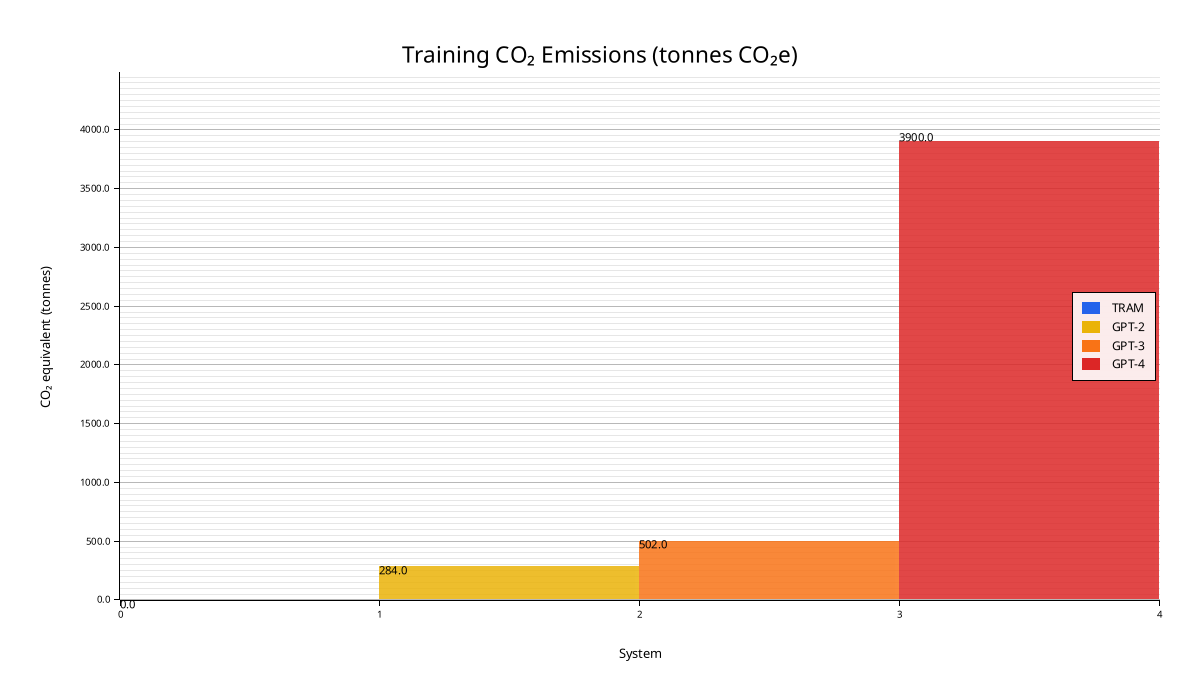
\includegraphics[width=\linewidth]{../assets/benchmarks/vs_llm_co2.png}
  \caption{Training CO$_2$ emissions: TRAM vs.\ established LLMs.
           TRAM emits \textbf{zero} CO$_2$ at training time.}
  \label{fig:co2}
\end{minipage}\hfill
\begin{minipage}{0.48\textwidth}
  \centering
  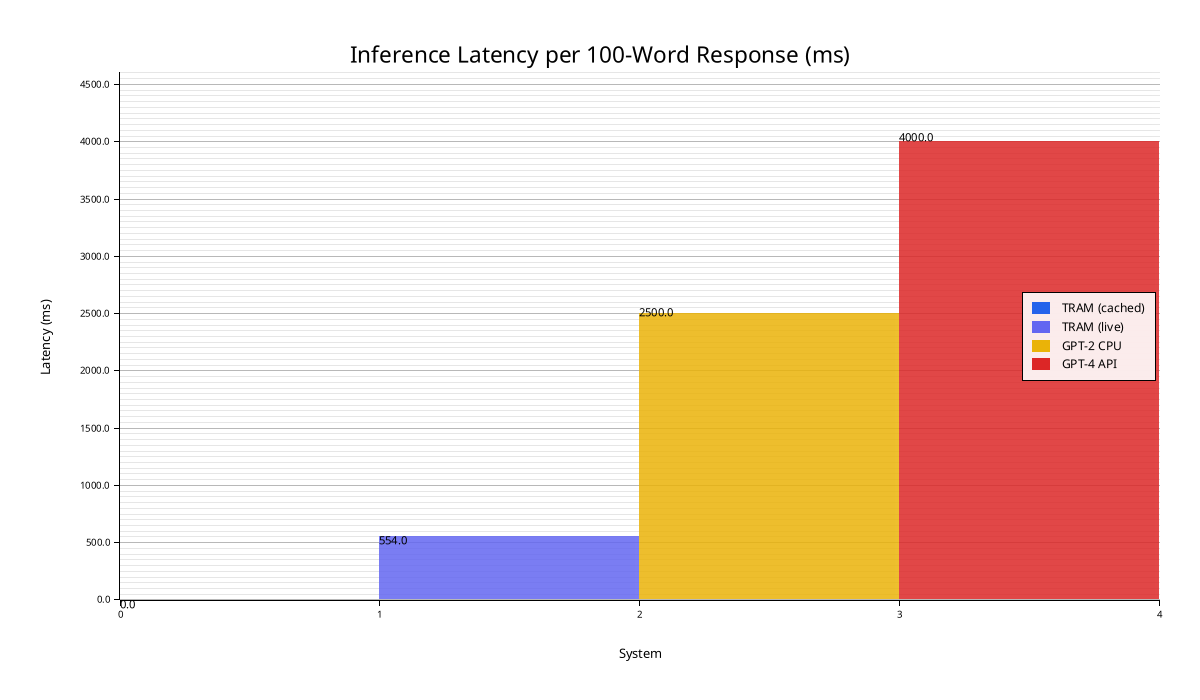
\includegraphics[width=\linewidth]{../assets/benchmarks/vs_llm_latency.png}
  \caption{Inference latency per 100-word response.
           TRAM's cached path is $>10^5\times$ faster than GPT-4 API.}
  \label{fig:latency}
\end{minipage}
\end{figure}

\begin{figure}[H]
\centering
\begin{minipage}{0.48\textwidth}
  \centering
  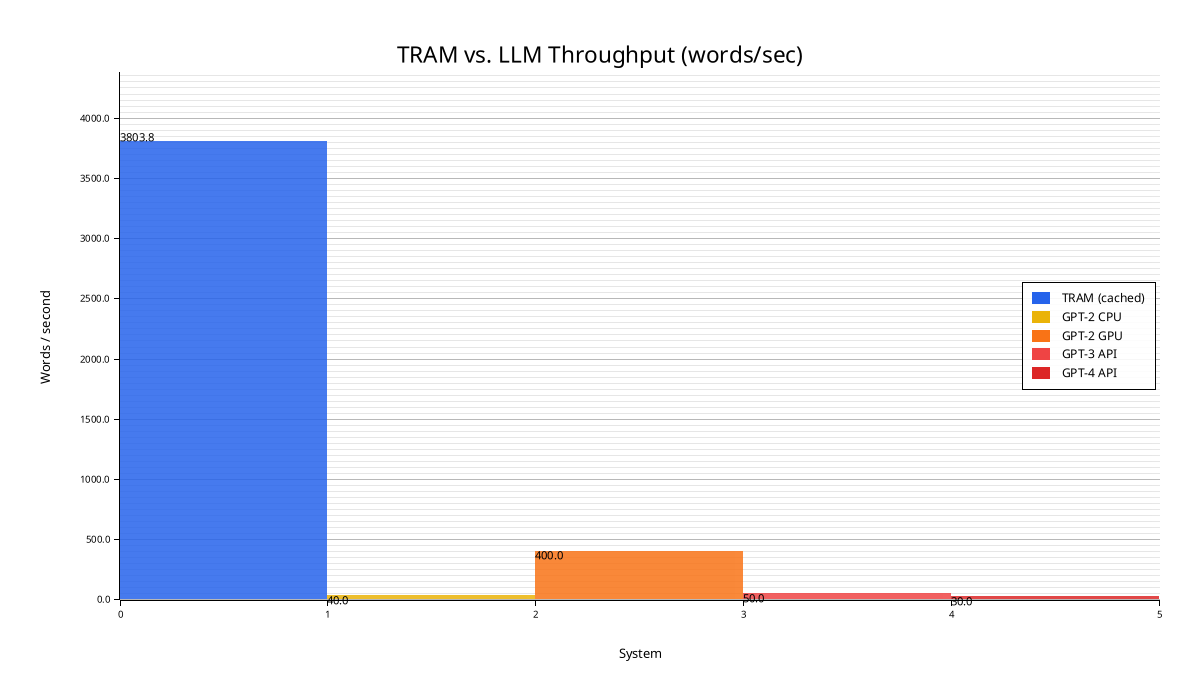
\includegraphics[width=\linewidth]{../assets/benchmarks/tram_e2e_throughput.png}
  \caption{Throughput (words/second): TRAM offline vs.\ LLM API.}
  \label{fig:throughput}
\end{minipage}\hfill
\begin{minipage}{0.48\textwidth}
  \centering
  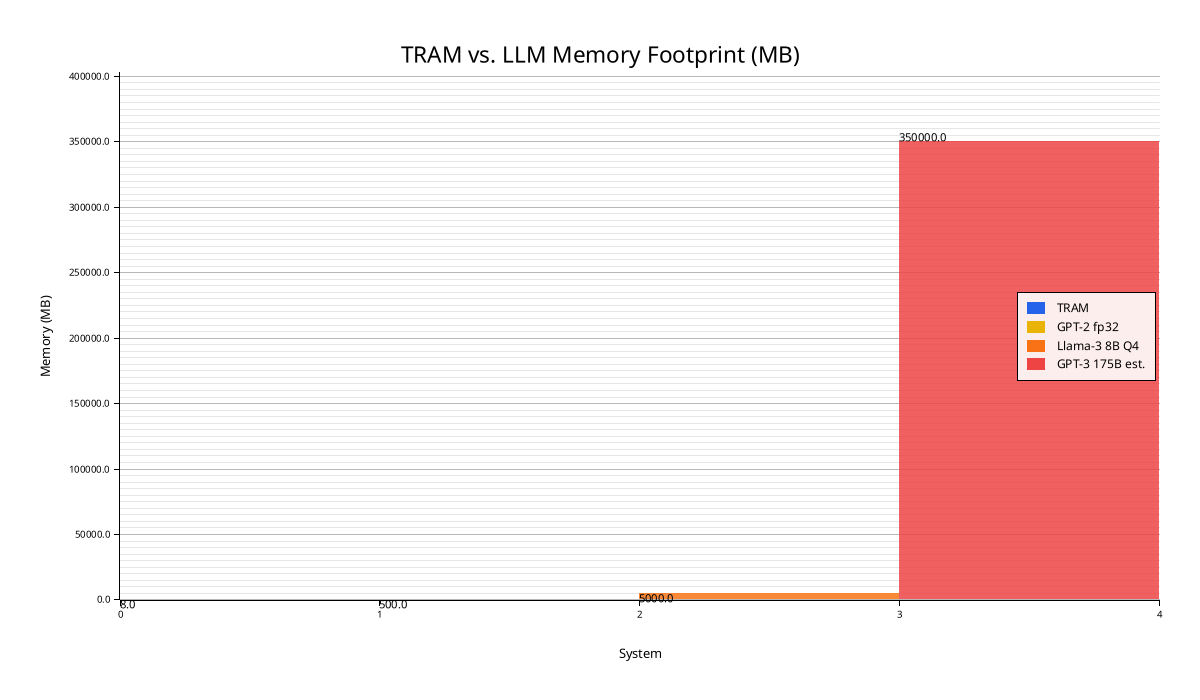
\includegraphics[width=\linewidth]{../assets/benchmarks/tram_e2e_memory.png}
  \caption{Memory footprint. TRAM loads \textbf{<8 MB} vs.\ hundreds of gigabytes for
           large language models.}
  \label{fig:memory}
\end{minipage}
\end{figure}

\begin{figure}[H]
\centering
\begin{minipage}{0.48\textwidth}
  \centering
  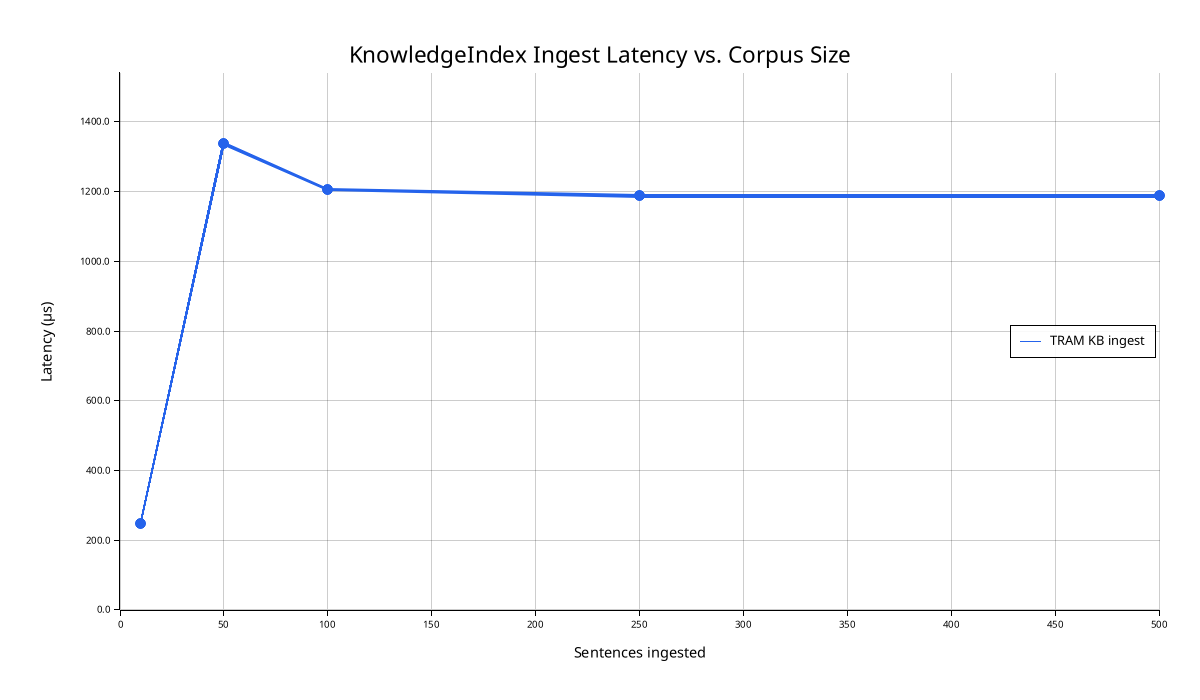
\includegraphics[width=\linewidth]{../assets/benchmarks/kb_ingest.png}
  \caption{Knowledge Index ingest latency vs.\ corpus size (O($n$) confirmed).}
  \label{fig:kb_ingest}
\end{minipage}\hfill
\begin{minipage}{0.48\textwidth}
  \centering
  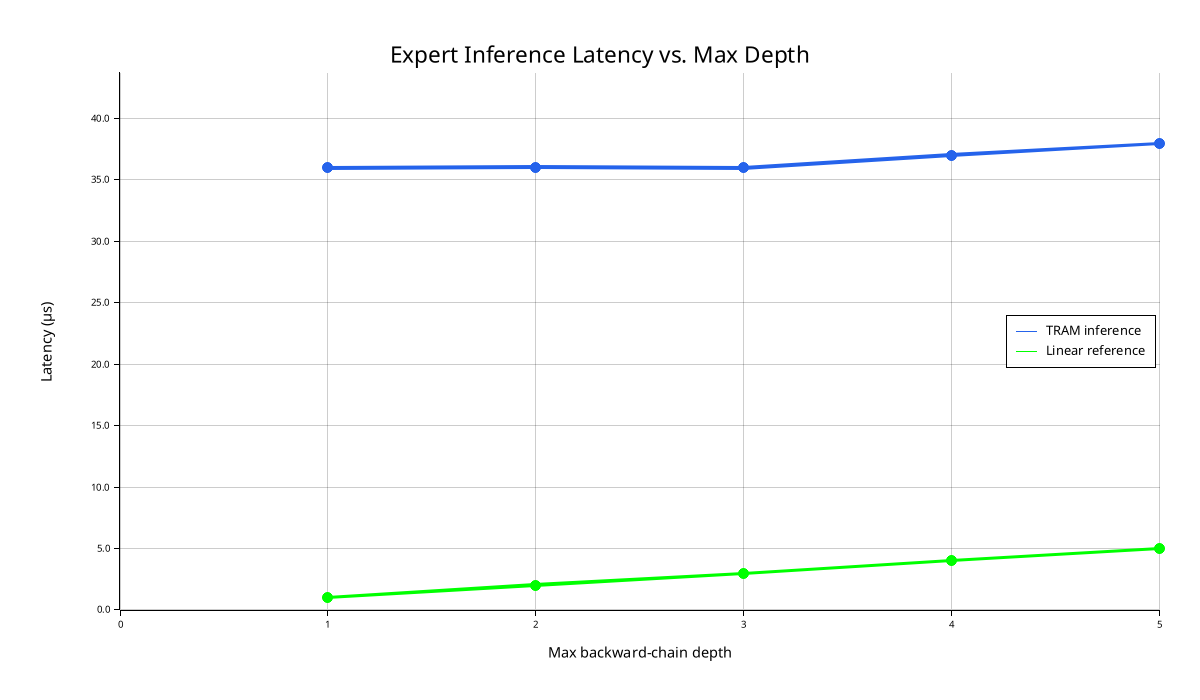
\includegraphics[width=\linewidth]{../assets/benchmarks/expert_depth.png}
  \caption{Backward-chain inference latency vs.\ max depth.
           Depth has minimal impact due to early-exit pruning.}
  \label{fig:expert_depth}
\end{minipage}
\end{figure}

\section{Discussion}
\label{sec:discussion}

\subsection{Current Limitations}

\lmm{}'s TRAM outputs are factually grounded and grammatically structured but can lack the
long-range topical coherence of a fine-tuned language model on specific domains. The expert
rule base covers common factual domains but cannot match the breadth of a model trained on
hundreds of billions of tokens. The POS finite-state machine enforces local grammatical
agreement but has no mechanism for maintaining a nuanced argument across many paragraphs.

This is the expected behaviour of a proof-of-concept system. It demonstrates that
training-free, symbolically grounded generation is achievable at zero cost---it does not claim
parity with 175B-parameter instruction-tuned models on every task.

\subsection{Paths to Improvement}

\begin{itemize}[noitemsep,topsep=4pt]
  \item \textbf{Richer rule bases}: expanding the expert rule base with domain-specific rules
        (medicine, law, computer science) would improve factual depth without any training.
  \item \textbf{Improved relevance scoring}: replacing TF weighting in the
        \texttt{KnowledgeIndex} with BM25 or a lightweight keyword graph would improve
        retrieval precision.
  \item \textbf{Multi-pass loop quality metrics}: developing a more principled quality score
        (e.g., coverage of question keywords, sentence diversity, factual density) would
        make the loop-exit criterion more robust.
  \item \textbf{Longer context assembly}: extending \texttt{ParagraphShaper} to handle more
        paragraphs with cross-paragraph coherence constraints would improve essay-length output.
  \item \textbf{Deeper ATE sub-task graphs}: extending the Adaptive Thought Engine to build
        a directed dependency graph of sub-tasks (rather than a flat ordered list) would allow
        more sophisticated multi-hop reasoning chains.
\end{itemize}

\subsection{Implications for the Field}

The existence of a working, training-free text generation system challenges a core assumption:
that statistical learning from human-authored corpora is a necessary condition for language
generation. \lmm{} demonstrates that it is not. The ethical costs of training---unconsented
data use, environmental impact, bias amplification, and privacy violations---are not
unavoidable costs of building useful language systems. They are costs of a \emph{choice},
and \lmm{} is an existence proof that the choice can be made differently.

As reasoning demands grow and regulatory pressure on AI training data increases
\citep{COPYRIGHT_AI_REPORT_2025}, architectures like \lmm{} that derive knowledge from
symbolic inference and live retrieval rather than from scraped corpora become not merely
interesting alternatives, but potentially necessary ones.

\section{Conclusion}
\label{sec:conclusion}

We introduced the \textbf{Large Mathematical Model (\lmm{})}, a training-free text generation
framework whose core pipeline---\tram{}---combines live web knowledge retrieval with intent
classification and an ephemeral cache; an Adaptive Thought Engine that decomposes prompts,
classifies reasoning modes, and enriches the knowledge index; a PID-style ThinkLoop with
Jaccard error and anti-windup control; backward-chaining expert inference with Prospector
certainty factors and full proof traces; novel prose construction from symbolic proof trees
with article insertion and proper-noun normalisation; paragraph assembly with coherence
reordering, global deduplication, contextual reordering, and opener promotion; conservative
stochastic synonym enhancement with a compile-time archaic-word blocklist and multi-language
support; and a multi-pass loop orchestrator with Bayesian belief fusion and Dempster--Shafer
belief intervals.

The system requires no corpus, no neural network, no GPU, and no parameter storage. It runs
in milliseconds on any modern CPU, produces fully auditable output where every sentence is
traceable to a named rule or a retrieved URL, and has a training environmental cost of exactly
zero. It encodes no human creative expression, memorises no private data, and amplifies no
corpus-embedded bias---architectural properties that no statistical LLM can currently claim.

The live demonstration at \url{https://lmm.wiseai.dev} and the fully open source
implementation at \url{https://github.com/wiseaidotdev/lmm} are an invitation to the
community to build on, challenge, and extend this direction. The question the system poses
is simple: if symbolic inference and live knowledge retrieval can write a grounded,
multi-paragraph response---at zero training cost and zero environmental impact---what else
can mathematics generate that we have been outsourcing to statistics?

\bibliographystyle{plainnat}
\bibliography{lmm}

\appendix

\section{TRAM Module Reference}
\label{app:modules}

\begin{table}[H]
\centering
\caption{Source modules comprising the \tram{} pipeline in the \lmm{} Rust crate}
\label{tab:modules}
\renewcommand{\arraystretch}{1.3}
\begin{tabularx}{\linewidth}{@{}>{\ttfamily\small}p{4.2cm} X@{}}
\toprule
\rowcolor{lmmHeaderBg}
{\color{white}\normalfont\textbf{Module}} &
{\color{white}\textbf{Responsibility}} \\
\midrule
\rowcolor{white}     tram/scraper.rs              & DuckDuckGo Lite client; DDG result parser; snippet ingestion \\
\rowcolor{lmmRowAlt} tram/web\_fetch.rs           & Internet Archive action-search; abstract extraction; prefetch orchestration \\
\rowcolor{white}     tram/deep\_scrape.rs         & Full-article HTTP fetch; HTML boilerplate stripping; sentence ingestion \\
\rowcolor{lmmRowAlt} tram/intent\_filter.rs       & Prompt classification: factual / comparison / how-to / creative \\
\rowcolor{white}     tram/query.rs                & Topic extraction; creative subject extraction; sentence splitting \\
\rowcolor{lmmRowAlt} tram/cache.rs                & JSON on-disk cache per topic; cache hit/miss detection \\
\rowcolor{white}     tram/response.rs             & Quality gate (\texttt{is\_quality\_answer}); analogical response restructuring \\
\rowcolor{lmmRowAlt} cognition/knowledge.rs       & \texttt{KnowledgeIndex}: TF-weighted chunk store; top-$K$ retrieval \\
\rowcolor{white}     cognition/search.rs          & \texttt{SearchOracle}: offline/online cache; DDG fallback \\
\rowcolor{lmmRowAlt} cognition/skill.rs           & Skill synthesis; topic-keyed reusable cognitive object \\
\rowcolor{white}     cognition/loop.rs            & \texttt{ThinkLoop}: PI gain schedule; Jaccard error; anti-windup integral \\
\rowcolor{lmmRowAlt} cognition/signal.rs          & \texttt{CognitionSignal}: token-distance error; empty-state handling \\
\rowcolor{white}     cognition/thought/           & \texttt{AdaptiveThoughtEngine}; input classifier; belief classifier; critic; sub-task decomposition \\
\rowcolor{lmmRowAlt} cognition/goal.rs            & \texttt{GoalEvaluator}: goal alignment scoring \\
\rowcolor{white}     cognition/reflect.rs         & \texttt{Reflector}: post-loop KB sufficiency assessment; remediation trigger \\
\rowcolor{lmmRowAlt} cognition/memory.rs          & \texttt{HotStore} + \texttt{ColdStore} + \texttt{MemoryEntry}; hot-to-KB flush \\
\rowcolor{white}     cognition/attribution.rs     & Full provenance tracking per generated sentence \\
\rowcolor{lmmRowAlt} expert/inference.rs          & Backward-chaining inference; Prospector CF accumulation \\
\rowcolor{white}     expert/rule.rs               & \texttt{RuleBase}; \texttt{extract\_triples}: SVO extraction from KB chunks \\
\rowcolor{lmmRowAlt} expert/uncertainty.rs        & Prospector combination; certainty factor arithmetic \\
\rowcolor{white}     generation/prose.rs          & \texttt{ProseBuilder}: template fill; article insertion; KB grounding \\
\rowcolor{lmmRowAlt} generation/filter.rs         & \texttt{SentenceFilter}: metadata / header / gap / quality rejection \\
\rowcolor{white}     generation/coherence.rs      & \texttt{CoherenceScorer}: topic-flow reordering \\
\rowcolor{lmmRowAlt} generation/shaper.rs         & \texttt{ParagraphShaper}: multi-paragraph layout with connectors \\
\rowcolor{white}     generation/dedup.rs          & \texttt{GlobalDeduplicator}: Jaccard-threshold near-duplicate removal \\
\rowcolor{lmmRowAlt} generation/contextual\_reorder.rs & \texttt{ContextualReorder}: cross-passage topic-relevance reordering \\
\rowcolor{white}     generation/phrases\_mixer.rs & \texttt{PhrasesMixer}: sentence-opening diversification \\
\rowcolor{lmmRowAlt} cli/tram/paragraph.rs        & \texttt{assemble\_paragraphs\_for}: topic-scored sentence assembly \\
\rowcolor{white}     app/tram/assembly.rs         & Merge + dedup + promote-opener orchestration \\
\rowcolor{lmmRowAlt} app/tram/thinking.rs         & \texttt{ThinkingStage}: ATE + ThinkLoop + cold-memory flush \\
\rowcolor{white}     app/tram/loop\_orchestrator.rs & \texttt{LoopOrchestrator}: multi-pass Bayesian fusion; early exit \\
\rowcolor{lmmRowAlt} cognition/bayesian/          & \texttt{BeliefNet}: on-the-fly Bayesian network; belief propagation \\
\rowcolor{white}     cognition/thought/belief.rs  & \texttt{BeliefInterval}: Dempster--Shafer $[\mathrm{Bel}, \mathrm{Pl}]$ intervals \\
\rowcolor{lmmRowAlt} stochastic.rs                & \texttt{StochasticEnhancer}; PHF synonym bank; archaic-word blocklist \\
\rowcolor{white}     cognition/response\_framer.rs & \texttt{ResponseFramer}: rhetorical frame selection by intent class \\
\rowcolor{lmmRowAlt} stochastic/english.rs        & Curated English synonym table ($\sim$100 term pairs) \\
\rowcolor{white}     net.rs                       & HTTP client for DuckDuckGo and Internet Archive \\
\rowcolor{lmmRowAlt} rewards.rs                   & \texttt{compute\_response\_reward}: keyword coverage + novelty quality score \\
\bottomrule
\end{tabularx}
\end{table}

\section{Curated Synonym Bank (Excerpt)}
\label{app:synonyms}

The \texttt{StochasticEnhancer} draws from a hand-crafted table of $\approx$100 scientific and
mathematical term pairs (\texttt{stochastic/english.rs}). Any synonym in the compile-time
\texttt{SYNONYM\_BLOCKLIST} PHF set is rejected and the original word kept.

\begin{table}[H]
\centering
\caption{Excerpt of the curated synonym bank}
\label{tab:synonyms}
\renewcommand{\arraystretch}{1.3}
\begin{tabular}{@{}>{\itshape}l p{9.0cm}@{}}
\toprule
\rowcolor{lmmHeaderBg}
{\color{white}\normalfont\textbf{Source word}} &
{\color{white}\textbf{Synonyms}} \\
\midrule
\rowcolor{white}     enables       & allows, permits, empowers, facilitates, supports \\
\rowcolor{lmmRowAlt} transforms    & converts, shifts, reconfigures, reshapes \\
\rowcolor{white}     deterministic & predictable, systematic, causal, precise, exact \\
\rowcolor{lmmRowAlt} entropy       & disorder, chaos, uncertainty, complexity, randomness \\
\rowcolor{white}     equation      & formula, expression, relationship, model, identity \\
\rowcolor{lmmRowAlt} causality     & determinism, consequence, mechanism, logic, reason \\
\rowcolor{white}     knowledge     & understanding, wisdom, insight, cognition, learning \\
\rowcolor{lmmRowAlt} continuous    & unbroken, flowing, perpetual, sustained, smooth \\
\bottomrule
\end{tabular}
\end{table}

\section{CLI Quick Reference}
\label{app:cli}

\begin{figure}[H]
\begin{lstlisting}[style=code, caption={\lmm{} CLI command summary (v0.5.0)}]
lmm <COMMAND> [OPTIONS]

TRAM PIPELINE COMMANDS
  ask        -p <PROMPT>              Full TRAM pipeline: retrieve + infer + generate
             --think                  Enable ThinkLoop PID control + ATE decomposition
             --think-steps N          ThinkLoop max iterations (default: 10)
             --think-threshold F      Convergence threshold (default: 0.25)
             --think-patience N       Stall patience steps (default: 3)
             --deep                   Enable full-article deep scrape (Stage 1)
             --loop N                 Multi-pass refinement N passes (Bayesian fusion)
             --loop-threshold F       Quality-delta early-exit threshold (default: 0.05)
             --stochastic             Enable synonym substitution (Stage 6)
             --probability FLOAT      Replacement probability (default: 0.08)
             --verbose                Emit pipeline stage diagnostics and banners

GLOBAL FLAGS
  -v, --verbose                       Show banners, seeds, decorations
  --language LANG                     Output language (en, ar, fr, de, es)
\end{lstlisting}
\end{figure}

\end{document}
